
\documentclass[12pt,reqno]{article}

\usepackage[a4paper,top=1.2in, left=0.9in]{geometry}
\usepackage{pgfplots}
\usepackage{setspace}
\pgfplotsset{compat=1.15}
\usepackage{amssymb}
\usepackage{amsmath}
\usepackage{amsthm}
\usepackage{mathrsfs}
\usepackage{circuitikz}
\usepackage{caption}
\usepackage{subcaption}
\usepackage{xcolor}
\usepackage{enumitem}
\usepackage{float}
\usepackage{hyperref}

\newtheorem{Thm}{Theorem}[section]
\newtheorem{lemma}[Thm]{Lemma}
\newtheorem{Prop}[Thm]{Proposition}
\newtheorem{Cor}[Thm]{Corollary}
\newtheorem{Rem}[Thm]{Remark}
\newtheorem{Def}[Thm]{Definition}
\newtheorem{Ex}[Thm]{Example}
\newtheorem{Claim}[Thm]{Claim}
\newtheorem{cor}[Thm]{Corollary}

\newtheorem{problem}{Problem}
\newtheorem*{solution}{Solution}

\newcommand{\tb}[1]{\textbf{#1}}
\newcommand{\np}{\newpage}
\newcommand{\tab}{\;\;\;\;\;\;}

\begin{document}
% \begin{center}
% {\LARGE\textbf{COMP4541 - Blockchain, Cryptocurrencies \& Smart Contracts }} \\
% \vspace{1cm}
% {\LARGE \textbf {Project Report}}\
% \vspace{1cm}

% \large \textbf{Name:}
% \underline{HASAN, Dewan Saadman}
% \hfill 
% \textbf{Student ID:} 
% \underline{20920414}

% \noindent\rule{12cm}{0.4pt}
% \end{center}

\pagenumbering{gobble}

\vspace*{\fill}
\begin{center}
    \begin{huge}
        \textbf{SPRING 2024-25 COMP 4541} \\
        \vspace{0.5cm}
        \textbf{Decentralized Crowdfunding Platform} \\
    \end{huge}
    \vspace{0.5cm}
    Name: HASAN, Dewan Saadman \tab \tab SID: 20920414
\end{center}
\vspace*{\fill}

%%%%%%%%%%%%%%%%%%%%%%%%%%%%%%%%%%%%%%%%%%%%%%%%%%%%%%%%%%%%%%%%%%%%%%%%%%%%

\np
\tableofcontents

%%%%%%%%%%%%%%%%%%%%%%%%%%%%%%%%%%%%%%%%%%%%%%%%%%%%%%%%%%%%%%%%%%%%%%%%%%%%

\np
\pagenumbering{arabic}
\section{Introduction}
Crowdfunding is a method for individuals, startups, and organizations to 
raise funds for their projects or ventures by soliciting small contributions 
from online communities. It provides a platform for creators and entrepreneurs 
to showcase their ideas and turn them into reality without traditional funding 
methods like bank loans or venture capital, or to raise funds for charitable 
causes, personal projects, or community initiatives. Through crowdfunding, backers, 
or contributors, donate small amounts of money to support a project, 
often in exchange for rewards, equity, or other incentives. \\ 
\newline 
Crowdfunding has gained immense popularity in recent years, with platforms like 
Kickstarter, Indiegogo, GoFundMe, and Patreon leading the way. These platforms, 
although different in their approaches, all share the common goal of connecting 
creators with potential backers. For example, Kickstarter focuses on funding 
creative projects like art, music, film, games through their all-or-nothing funding model, 
while GoFundMe is more geared towards personal causes and charitable fundraising. Patreon, 
on the other hand, allows creators to earn recurring income by offering exlusive 
content and perks to their subscribers. \\ 
\newline 
In view of this idea, we build a decentralized crowdfunding platform on the 
Ethereum testnet. The platform allows users to create and fund projects by calling 
a smart contract. The smart contract is deployed on the Ethereum blockchain. Similar to 
Kickstarter, we employ an all-or-nothing funding model, where the project creator 
must reach their funding goal within a specified time frame. If the goal is not met, 
the funds are returned to the contributors. In addition, we propose a voting-based 
mechanism to allow the community to decide whether the creator would be able to withdraw 
the fund before the goal and time limit is reached.  

\newpage

\section{Contract Functionality}
In this section we will discuss the functionality of our smart contract. The contract is 
written in Solidity and is deployed on the Ethereum testnet. The contract has two types of 
users: the project or campaign creators and the contributors, who donote to the projects. The 
contract has the following functionalities: \\

\subsection{Create Campaign}
The project creator can create a campaign by calling the \texttt{createCampaign} function. It takes 
the following parameters: \\ 
\begin{itemize}
    \item \texttt{title}: The title of the campaign.
    \item \texttt{description}: A brief description of the campaign.
    \item \texttt{goalAmount}: The funding goal for the campaign.
    \item \texttt{durationinDays}: The duration of the campaign in number of days.
    \item \texttt{image} (optional): The URL of the campaign image.
\end{itemize}

\subsection{Campaign Details}
Once created, a campaign is assigned a unique ID and is stored in the contract's mapping. 
A campaign stores the following additional information: \\ 
\begin{itemize}
    \item \texttt{creator}: The address of the project creator.
    \item \texttt{fundsRaised}: The total amount of ETH raised for the campaign.
    \item \texttt{goalReached}: A boolean value indicating whether the amount raised met the goal or not.
    \item \texttt{isWithdrawn}: A boolean value indicating whether the funds have been withdrawn or not.
    \item \texttt{yesbeforegoal}: An int value indicating weighted vote in favour of early withdrawal.
    \item \texttt{totalvotes}: An int value indicating total votes for early withdrawal.
    \item \texttt{withdrawnbeforegoal}: A boolean value indicating early withdrawal.
    \item \texttt{afterwithdraw}: Contributor address mapping to boolean value indicating whether the 
    contribution was made after the early withdrawal or not 
    \item \texttt{contributors}: An array of addresses of contributors who have donated to the campaign.
    \item \texttt{contributions}: A mapping of contributor addresses to their respective contributions.
\end{itemize}
The campaign model is based on all-or-nothing funding model, where the project must reach its goal 
limit within the specified time frame. If the goal is not met, the contributors can call a function 
to get their funds back. However, we allow each campaign to withdraw the funds before the goal is 
reached at most one time. This process is voting based; when contributors donate to the campaign, 
they can choose to vote in favour of early withdrawal. The votes are weighted based on the amount 
contributed, which is indicated by \texttt{yesbeforegoal}. Early withdrawal is allowed if the number of 
yes votes is greater than half of the total votes, and possible only once throughout the entire duration 
of the campaign. Additionally, once the campaign deadline has passed, it will not be possible to 
withdraw partial funds in the event that the goal is not met. \\ 

\subsection{Contribution}
Contributors can donate to the campaign by calling the \texttt{contribute} function. It has a unique 
parameter \texttt{canwithdrawbefore}, which indicates whether the contributor wants to vote in favour
of early withdrawal or not. If true, and the campaign has not been withdrawn early, the contributor's 
vote is counted towards the \texttt{yesbeforegoal} variable. The contributor's address is added to the
campaign contributors array, and the contribution amount is stored in the contributions mapping. 

\subsection{Withdraw Funds before Goal}
As mentioned earlier, the project creator can withdraw the funds before the goal is reached if the
voting is in favour of early withdrawal. The creator can call the \texttt{withdrawFundsBeforeGoal}
function, which checks if the early withdrawal is allowed. This goes through the following checks: \\ 
\begin{itemize}
    \item The creator of the campaign must be the one calling the function.
    \item The campaign must be active and is not called after the dealine. 
    \item Target amount is greater than the amount raised. Otherwise the creator can withdraw full amount 
    after the deadline. 
    \item Fund early withdrawal is allowed only once.
    \item The number of yes votes must be greater than half of the total votes.
\end{itemize}    
In this case, the funds are transferred to the creator's address, \texttt{fundsRaised} is set to zero, 
and the target amount is reduced to the amount raised. The \texttt{withdrawnbeforegoal} variable is set to true, and the contribution 
array is updated. Any more contributions made after the early withdrawal will be marked as true in the 
\texttt{afterwithdraw} mapping, so that the contributors can get their funds back if the end goal 
is not reached. 

\subsection{Withdrawing Funds After Deadline}
The project creator can withdraw the funds after the deadline by calling the \texttt{withdrawFunds}
function. It can only be activated if 
\begin{itemize}
    \item The creator of the campaign must be the one calling the function.
    \item The campaign deadline must have passed. 
    \item The campaign goal must be reached. 
    \item Funds must not have been fully withdrawn before. 
\end{itemize}
If the conditions are met, the funds are transferred to the creator's address, and the
variables are changed to indicate that the funds have been withdrawn. 

\subsection{Refunding Contributors}
Contributors can get their funds back by calling the \texttt{requestRefund} function. Refunds 
can be requested if the campaign deadline has passed and the goal has not been reached. The function 
also checks the \texttt{contributions} mapping to see if the contributor has made a contribution.
If the conditions are met, the function checks if the campaign has been withdrawn early. If the 
campaign has been withdrawn early and the contribution was made before the early withdrawal, the 
contributor will not be able to get a refund as the funds have already been withdrawn. Otherwise, 
funds are transferred back to the contributor's address, and the contribution amount is set to zero.

\subsection{Getting Campaign Details}
Campaign details can be retrieved by calling the \texttt{getCampaign} function, which returns 
the state of the campaign so far. 

\newpage

\section{Testing On Remix Virtual Machine}
We test the contract on Remix VM, since test faucets were not adequate to conduct testing 
on the Ethereum testnet. 

\subsection{Basic Functionalities}

The basic functionalities of the contract, namely campaign creation, 
making contributions, and campaign details are tested below: 

\begin{figure}[h!]
    \centering
    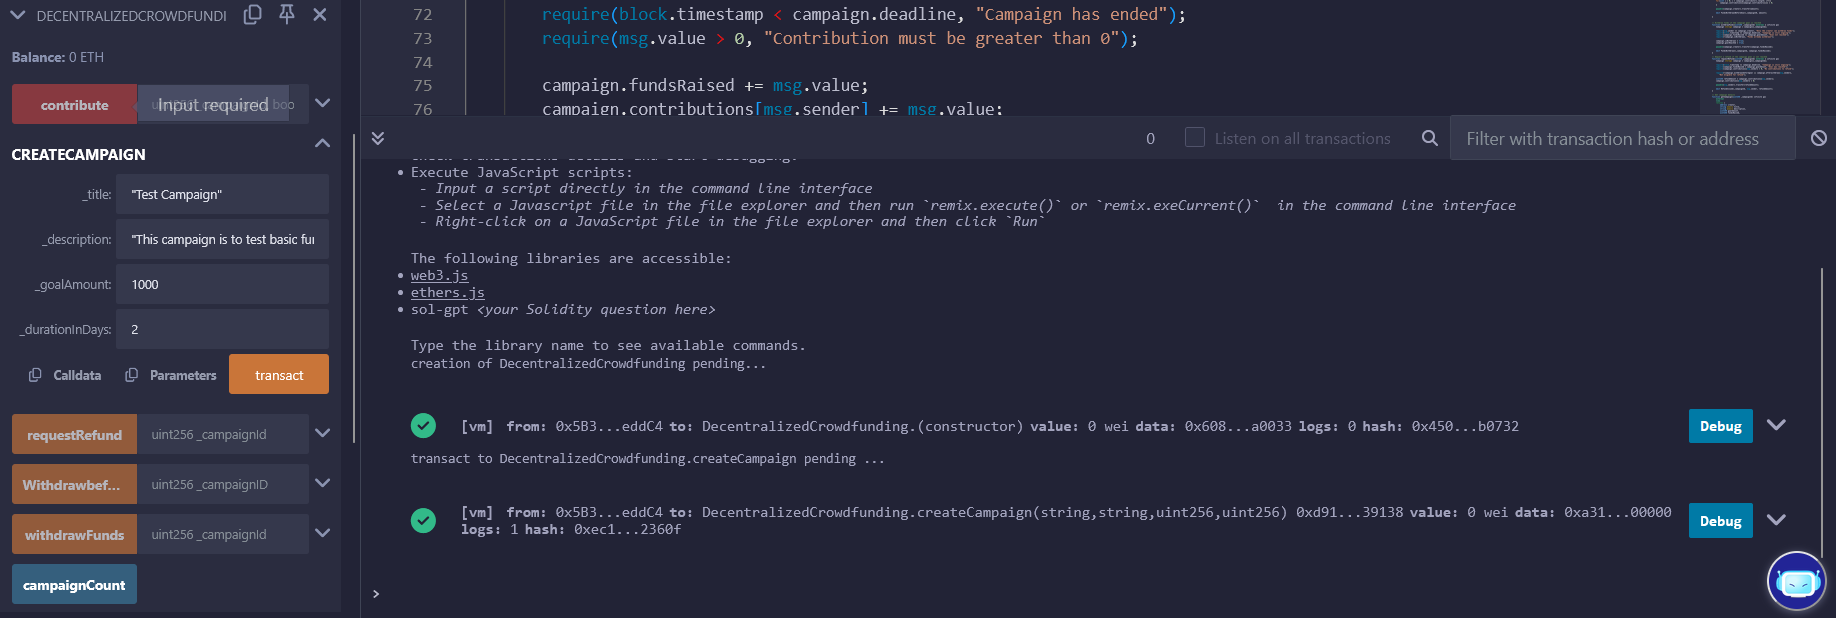
\includegraphics[width=0.6\linewidth]{Pictures/camp_create.png}
    \caption{Campaign Creation}
    \label{camp_create}
\end{figure}

\begin{figure}[h!]
    \centering
    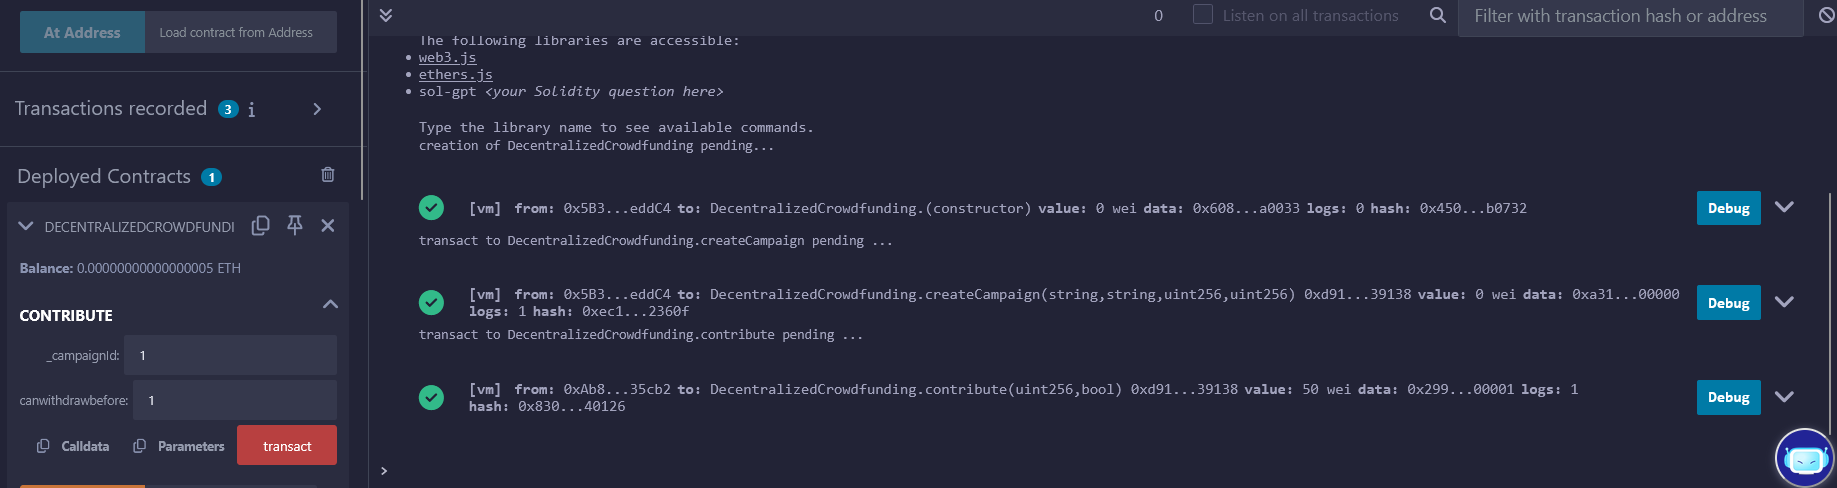
\includegraphics[width=0.6\linewidth]{Pictures/first_transaction.png}
    \caption{First transaction with yes vote}
    \label{first_transaction}
\end{figure}

\begin{figure}[h!]
    \centering
    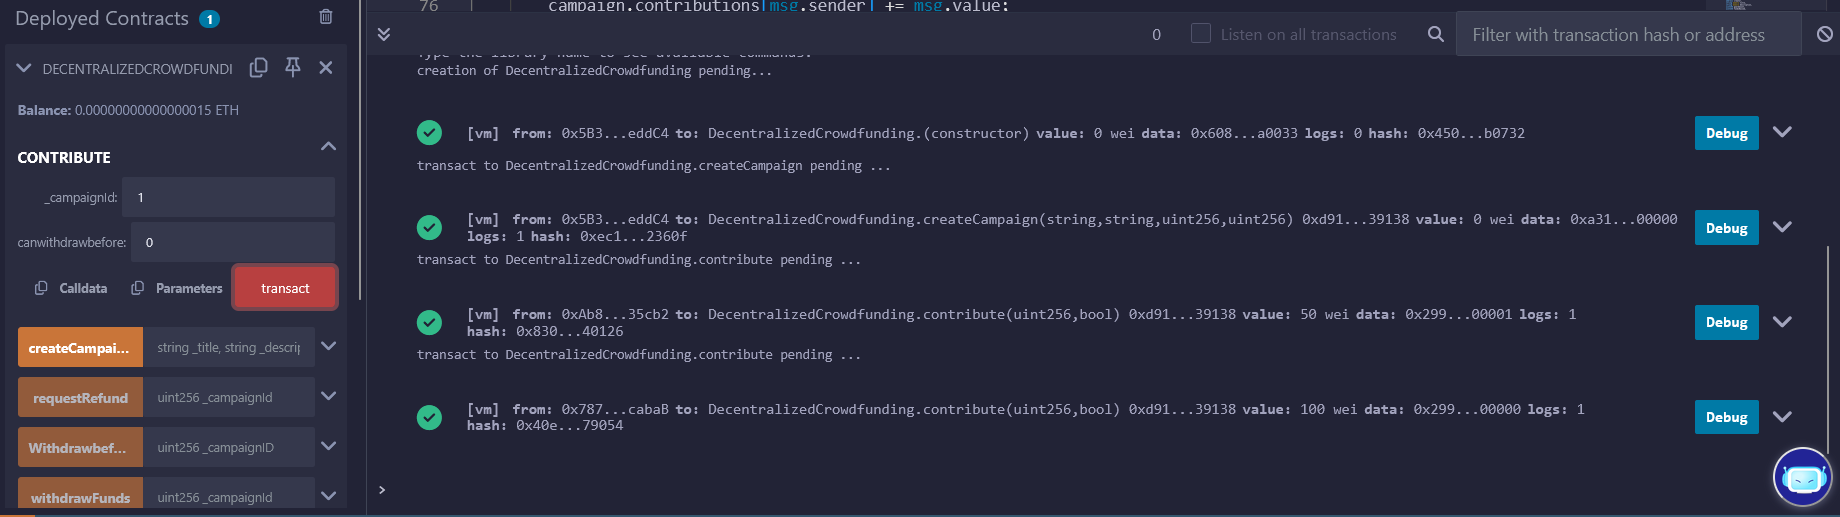
\includegraphics[width=0.6\linewidth]{Pictures/second_transaction.png}
    \caption{Second transaction with no vote}
    \label{second_transaction}
\end{figure}

\begin{figure}[!ht]
    \centering
    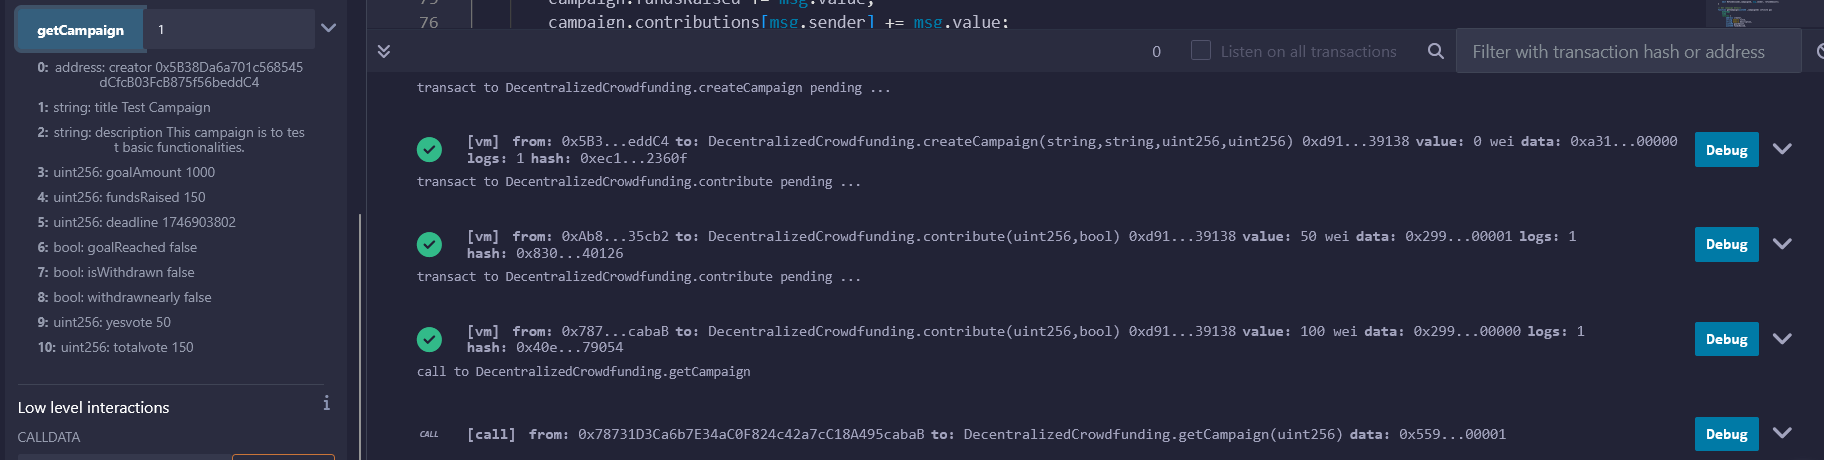
\includegraphics[width=0.6\linewidth]{Pictures/campaign_details.png}
    \caption{Campaign Details}
    \label{details}
\end{figure}

\newpage 

\subsection{Withdrawing Funds Before Goal}
Since the campaign has not reached its deadline, the creator can call early 
withdrawal. Since it requires specific percent of vote, it will fail as following: 
\begin{figure}[h!]
    \centering
    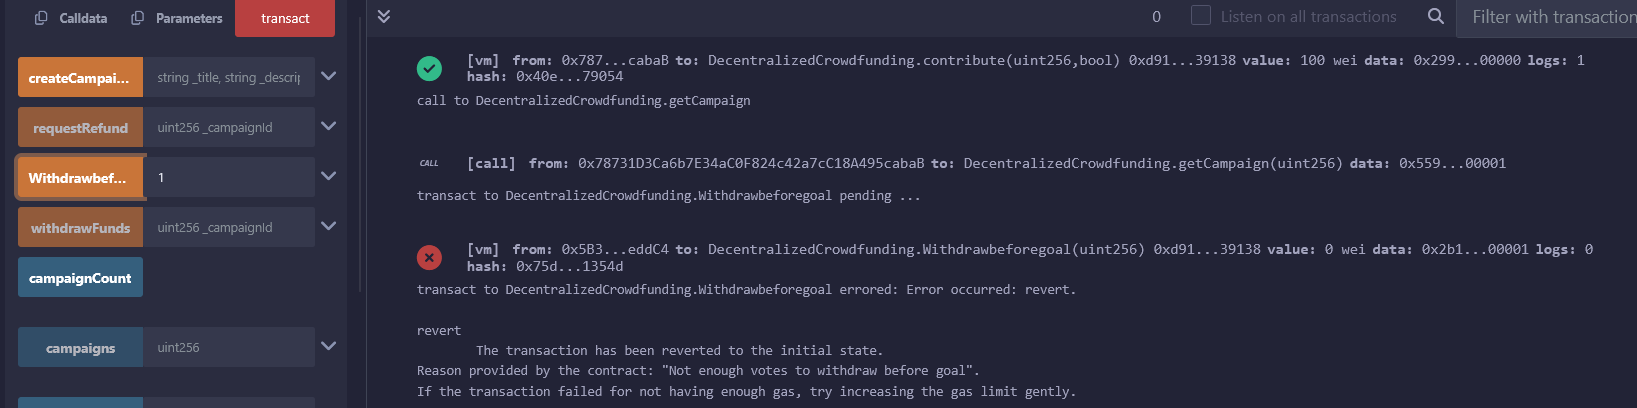
\includegraphics[width=0.6\linewidth]{Pictures/early_withdraw1.png}
    \caption{Early withdrawal failed}
    \label{early_withdraw1}
\end{figure}
Next, we will make another transaction with a yes vote with sufficient weight, and 
then call the early withdrawal function again.
\begin{figure}[h!]
    \centering
    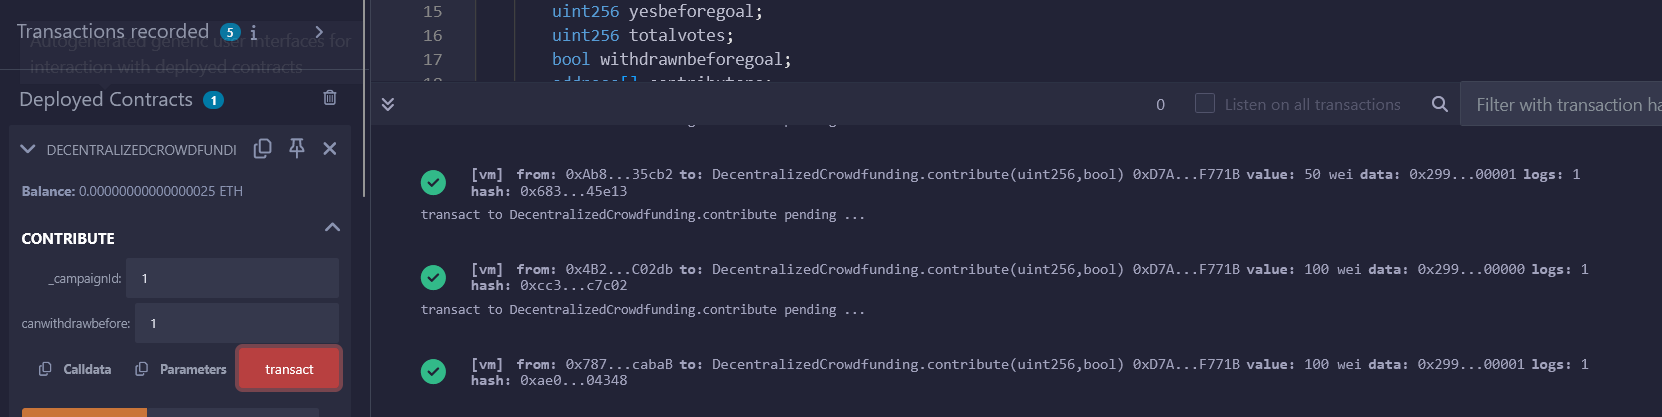
\includegraphics[width=0.6\linewidth]{Pictures/third_transaction.png}
    \caption{Third transaction with yes vote}
    \label{third_transaction}
\end{figure}

\begin{figure}[h!]
    \centering
    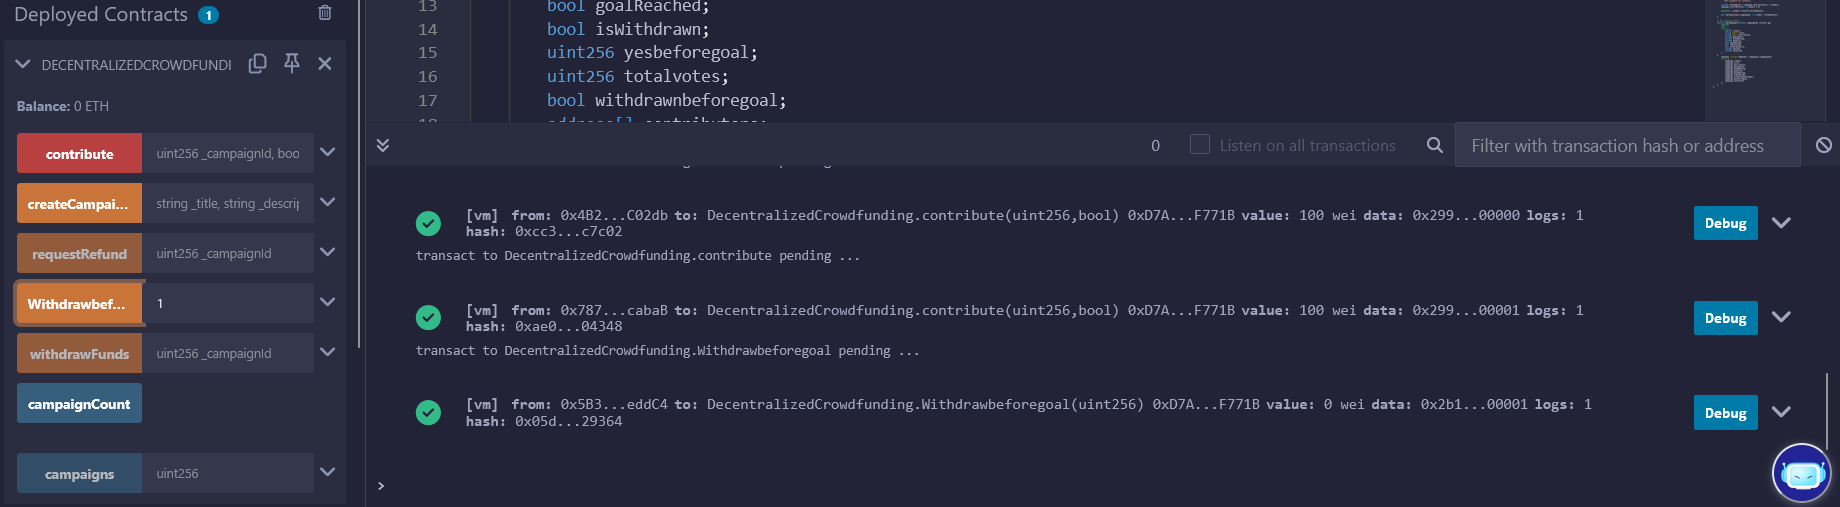
\includegraphics[width=0.6\linewidth]{Pictures/early_withdraw2.png}
    \caption{Successful early withdrawal}
    \label{early_withdraw2}
\end{figure}

We can see the campaign details have been updated to show that the funds have been withdrawn, 
and the target amount has been reduced. Next, we try to see if we can call 
the early withdrawal function again.

\begin{figure}[h!]
    \centering
    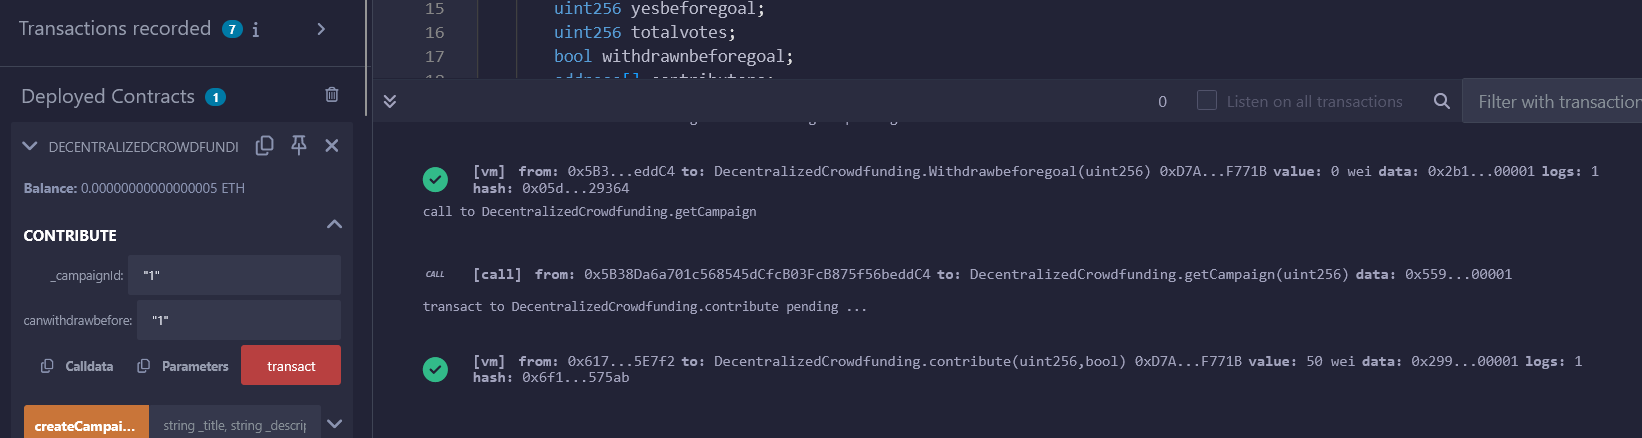
\includegraphics[width=0.6\linewidth]{Pictures/fourth_transaction.png}
    \caption{Fourth transaction with yes vote}
    \label{fourth_transaction}
\end{figure}
\newpage 
\newpage 
\begin{figure}[h!]
    \centering
    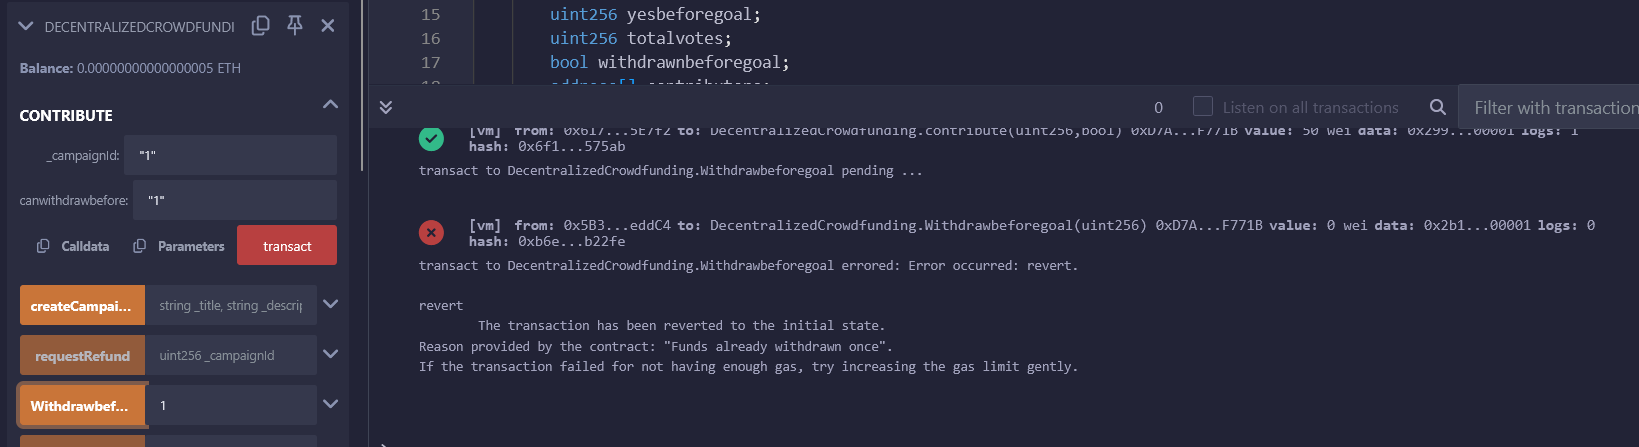
\includegraphics[width=0.6\linewidth]{Pictures/withdrawn_early.png}
    \caption{Second time early withdrawal failed}
    \label{withdrawn_early}
\end{figure}

\subsection{Refunding Contributors}
Contributors can only get their funds back only after the campaign 
deadline has passed. Contributors do not get their funding back if the 
campaign goal is reached at any point of time. 

\begin{figure}[h!]
    \centering
    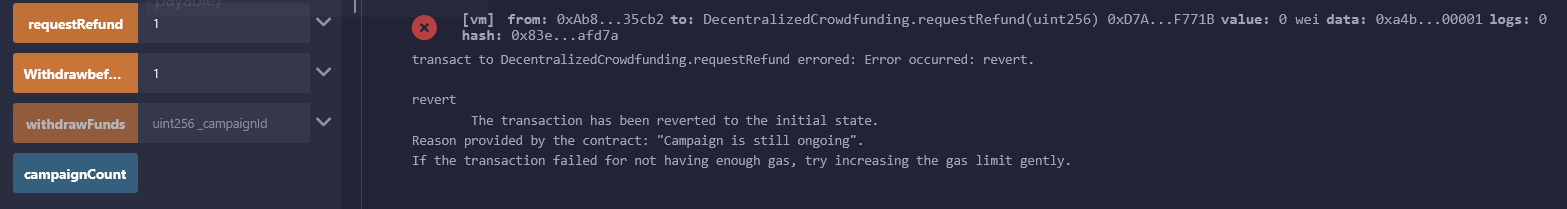
\includegraphics[width=\linewidth]{Pictures/failed_refund1.png}
    \caption{Campaign still active, refund failed}
    \label{failed_refund1}
\end{figure}

The process becomes a bit tricky if the campaign has been withdrawn early. 
In this case, only the contributors who made their contributions 
after the withdrawal can get their funds back, and can only be claimed 
after the deadline has passed and the goal has not been reached. 

\begin{figure}[h!]
    \centering
    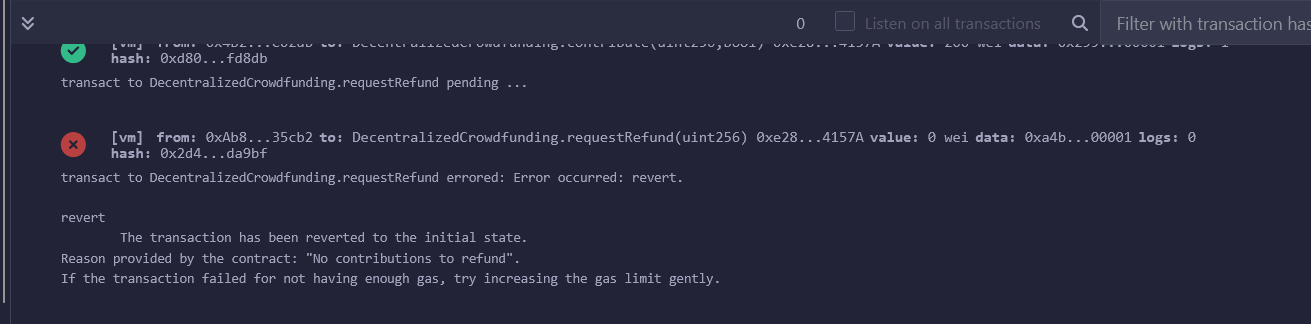
\includegraphics[width=0.6\linewidth]{Pictures/request_refund1.png}
    \caption{Refund failed because of early withdrawal}
    \label{refund1}
\end{figure}
Figure~\ref{refund1} shows that the contributor can get their funds 
back even though the campaign has been withdrawn early, because the 
contribution was made after the early withdrawal.

\begin{figure}[h!]
    \centering
    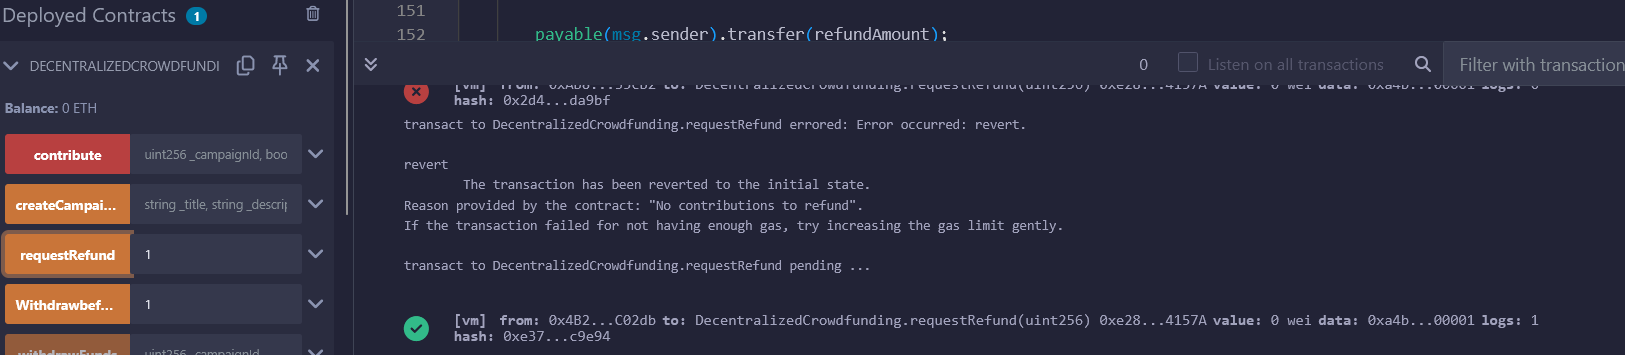
\includegraphics[width=0.6\linewidth]{Pictures/request_refund2.png}
    \caption{Successful refund after deadline and goal not reached}
    \label{refund2}
\end{figure}

\newpage
\subsection{Withdrawing Funds After Deadline}
Only the project creator can withdraw the funds after the deadline. 
In case the goal has not been reached, there is no way to withdraw 
the funds for the creator. 
\begin{figure}[h!]
    \centering
    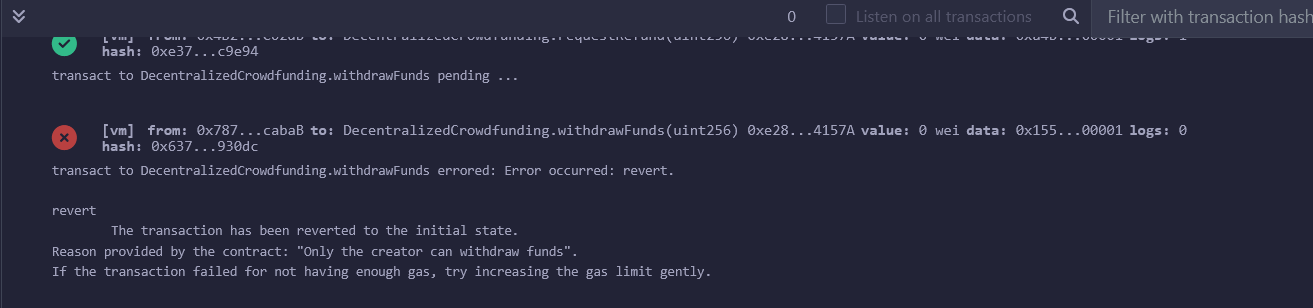
\includegraphics[width=0.6\linewidth]{Pictures/withdraw_late1.png}
    \caption{Only creators can withdraw funds after deadline}
    \label{withdraw_late1}
\end{figure}

\begin{figure}[h!]
    \centering
    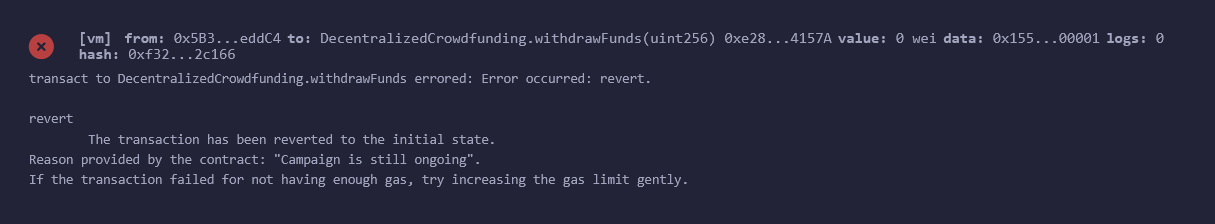
\includegraphics[width=0.6\linewidth]{Pictures/withdraw_late2.png}
    \caption{Cannot withdraw ongoing project}
    \label{withdraw_late2}
\end{figure}

\begin{figure}[h!]
    \centering
    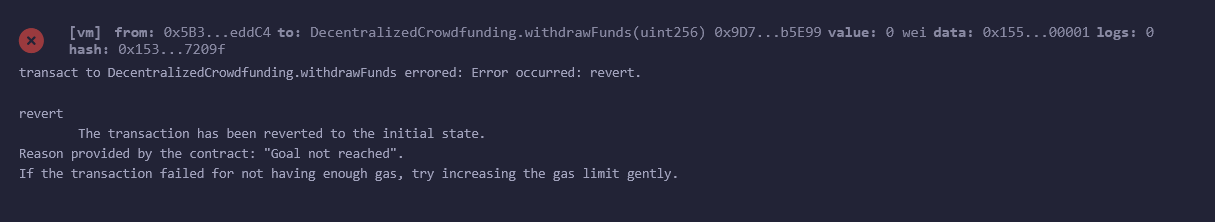
\includegraphics[width=0.6\linewidth]{Pictures/withdraw_late3.png}
    \caption{Cannot withdraw if goal has not been reached}
    \label{withdraw_late3}
\end{figure}

\begin{figure}[h!]
    \centering
    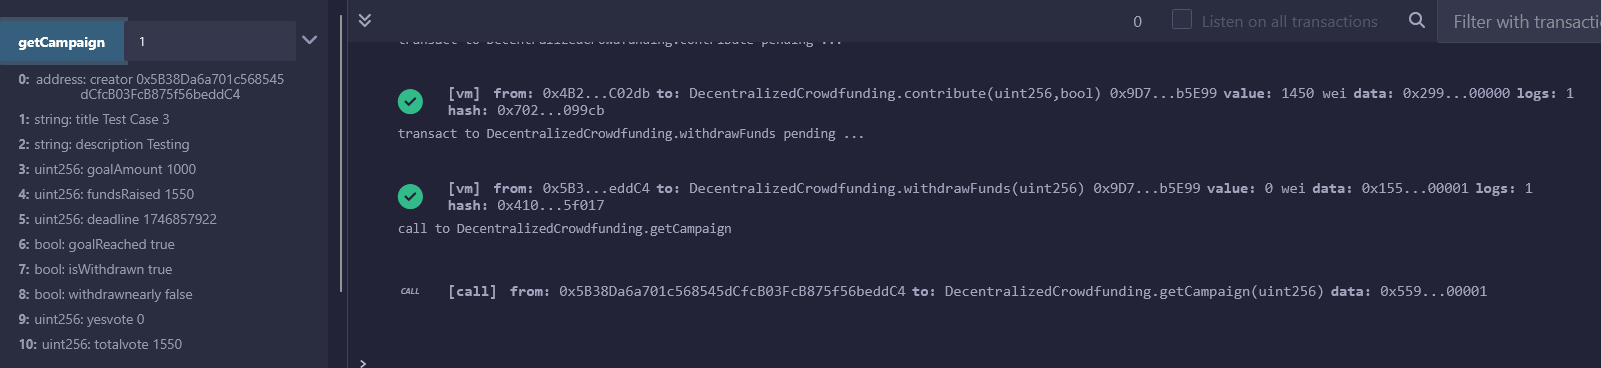
\includegraphics[width=0.6\linewidth]{Pictures/withdraw_late4.png}
    \caption{Successful withdrawal with project condition}
    \label{withdraw_late4}
\end{figure}

\begin{figure}[h!]
    \centering
    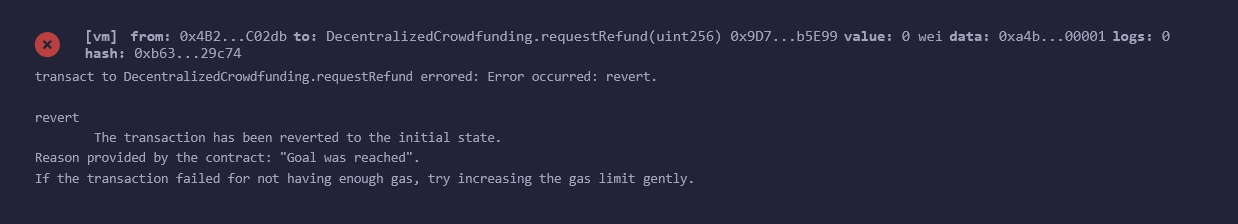
\includegraphics[width=0.6\linewidth]{Pictures/refund_req1.png}
    \caption{Unsucccessful refund request}
    \label{refund_failed1}
\end{figure}

\newpage 

\begin{figure}[h!]
    \centering
    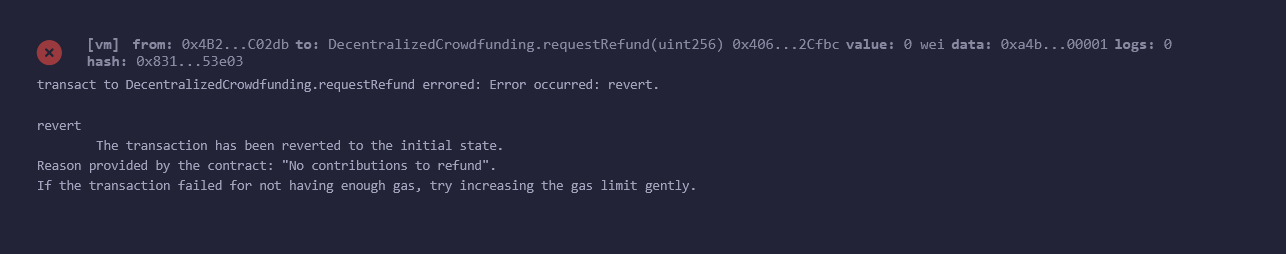
\includegraphics[width=0.6\linewidth]{Pictures/refund_req2.png}
    \caption{Cannot refund if no contribution made}
    \label{refund_failed2}
\end{figure}

\subsection{Other Security Checks}
The contract is secured against re-entrancy attacks by ensuring 
states ar updated before transferring funds. The contract also 
ensures that no token is stuck in the contract by validating who 
can donate and who can withdraw. 

\newpage

\section{User Interface}
We have built a simple user interface using html and javascript. 
The interface allows users to create campaigns, make contributions, 
withdraw funds (both before and after goal), and request refunds.  
Each campaign created is displayed on the interface, and potential 
contributors can see the details of the campaign, including 
goal amount, funds raised, time left for the campaign, vote percent 
for early withdrawal and so on. \\ 

The interface requires the user to connect to their MetaMask wallet 
before using the functionalities. Once connected, users will see the 
following screen: \\

\begin{figure}[h!]
    \centering
    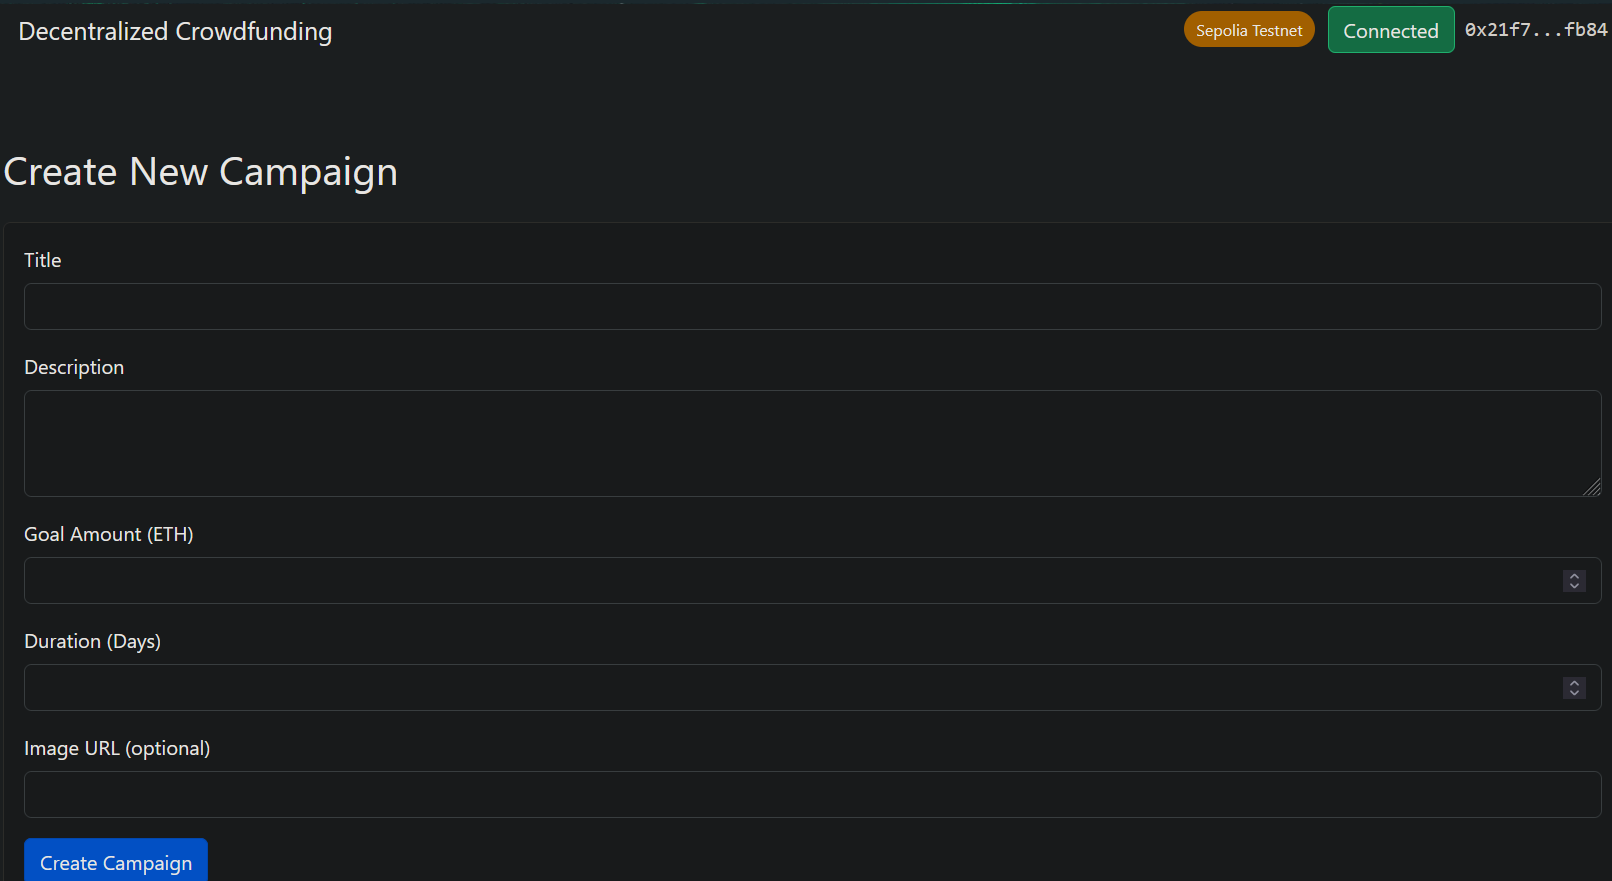
\includegraphics[width=0.6\linewidth]{Pictures/ui_1.png}
    \caption{User Interface, campaign creation}
    \label{cam_create}
\end{figure}

Project creators can fill up the required fields and create their 
campaign. Once created, the campaign will be displayed on the 
interface as soon as the transaction is confirmed. 

\begin{figure}[h!]
    \centering
    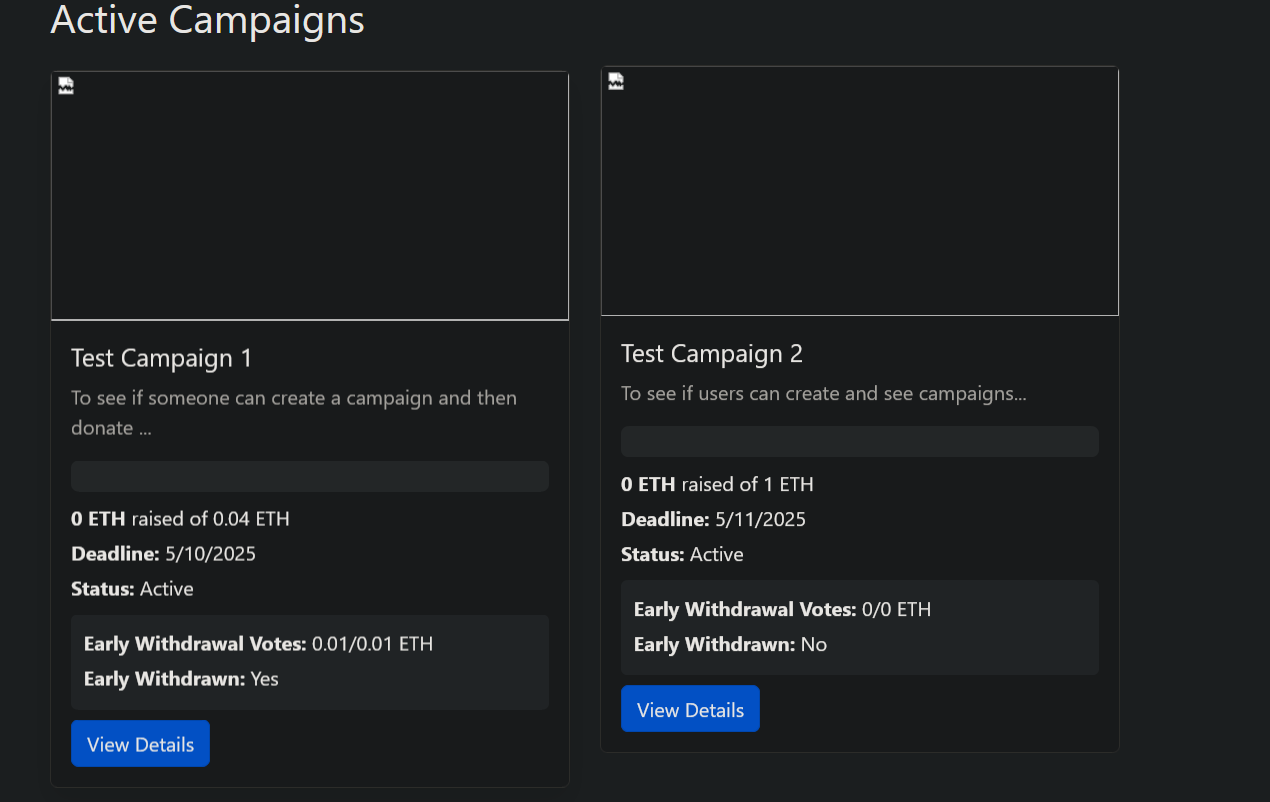
\includegraphics[width=0.6\linewidth]{Pictures/ui2.png}
    \caption{Available Campaigns}
    \label{cam_display}
\end{figure}

To donate to a campaign, the user can click on the 
\texttt{View Details} button, which will show the details 
of the campaign and the option to donate. The user can enter their 
contribution amount and choose whether they want to vote in favour 
of early withdrawal or not. Once the transaction is confirmed, 
updated campaign details will be displayed. In addition, before 
the deadline, the campaign create can withdraw the funds by clicking 
the \texttt{Withdraw Early} button. 

\begin{figure}[h!]
    \centering
    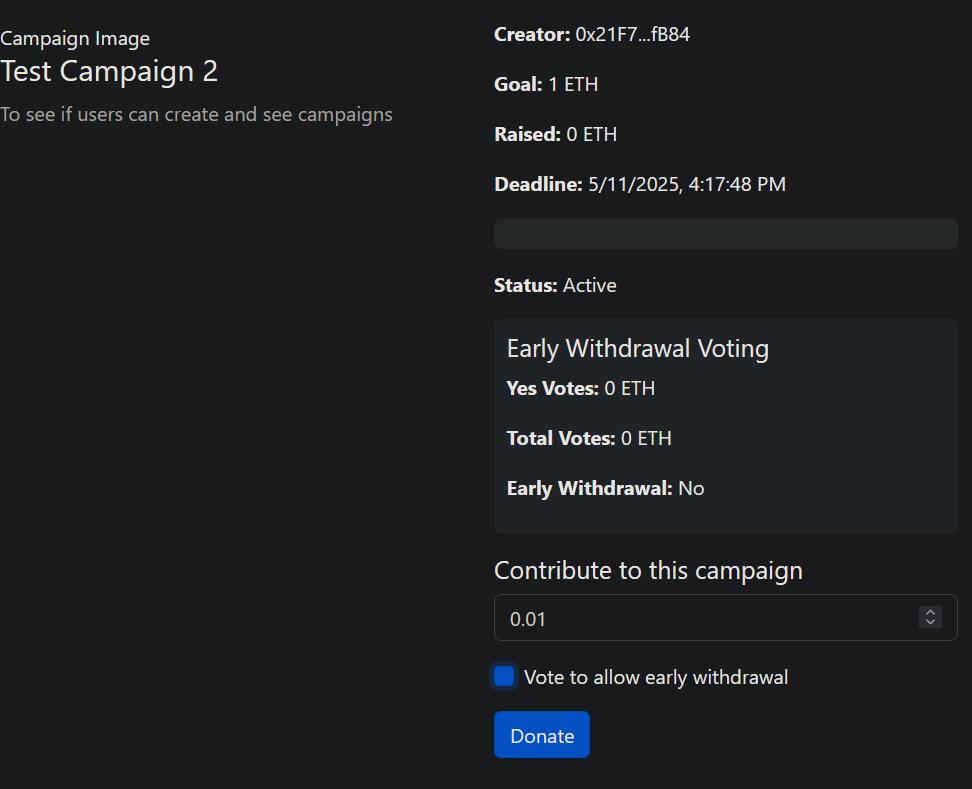
\includegraphics[width=0.6\linewidth]{Pictures/ui3.png}
    \caption{Donating to a campaign}
    \label{donation}
\end{figure}

\begin{figure}[h!]
    \centering
    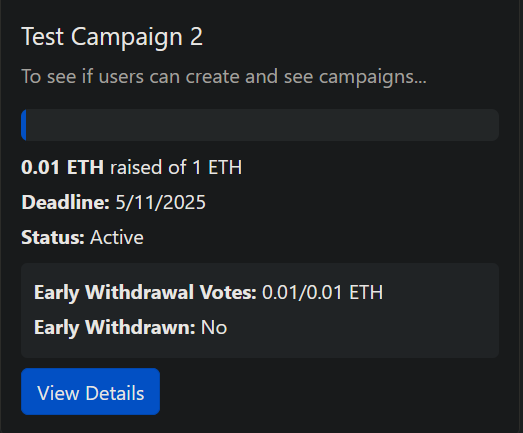
\includegraphics[width=0.6\linewidth]{Pictures/ui4.png}
    \caption{Updated Campaign details}
    \label{donation2}
\end{figure}

Once withdrawn early, the button will be disabled, and it will 
not be possible to call early withdrawal again. 

\newpage 
\begin{figure}[h!]
    \centering
    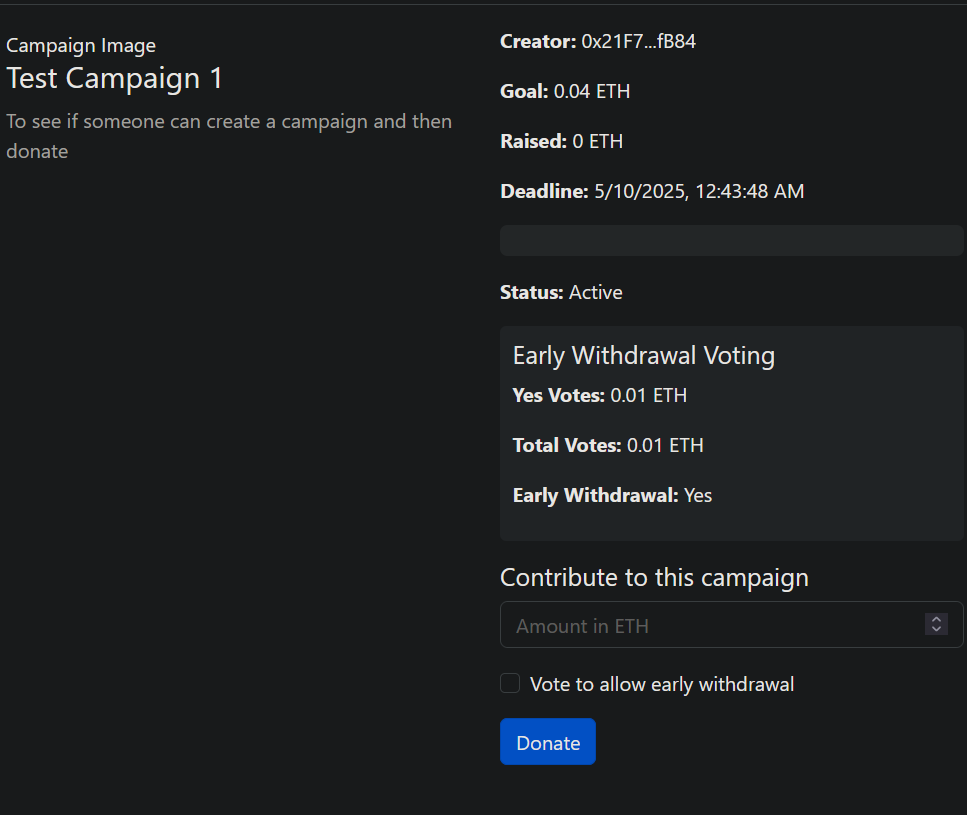
\includegraphics[width=0.6\linewidth]{Pictures/ui5.png}
    \caption{After early withdrawal}
    \label{after_early}
\end{figure}

Once the campaign deadline has passed, there will be option 
for the creator to withdraw the funds, and for the contributors 
to request their funds back. 

\section{Conclusion}
The Decentralized Crowdfunding with Early Withdrawal Voting 
smart contract represents a significant evolution in 
blockchain-based fundraising by introducing a flexible, 
trust-minimized system that balances the needs of both project 
creators and backers. With a fair voting mechanism, 
the contract empowers the community to make informed 
decisions about early fund withdrawals, ensuring that 
the interests of all parties are considered.  \\ 
\newline 
The early withdrawal system is designed to be transparent 
and secure, with clear rules and conditions for voting and fund 
withdrawal. This mechanism allows the project creator to access 
partial funds in the case of unmatched goals, while also 
penalizing greedy behavior. Since the early withdrawal call 
consumes more gas than the regular withdrawal, project creators 
are more incentized to withdraw the funds only when necessary. \\ 
\newline 
The user interface provides a seamless experience for both 
project creators and contributors, making it easy for anyone 
to call the contract functions. The integration with MetaMask 
and the Ethereum testnet allows users to interact with the
contract without the need for complex setups or technical
knowledge. \\
\newline 
While this contract provides a robust foundation, 
potential improvements include reducing costs for refund 
processing in high-participation campaigns, enabling contributions 
in stablecoins or other ERC-20 tokens, and
allowing backers to vote on fund releases at specific development 
stages.\\ 
\newline 
Finall, This smart contract successfully addresses a critical 
limitation in traditional crowdfunding—rigidity in fund 
access—by introducing a decentralized, vote-based withdrawal 
system. By empowering backers with governance rights while 
protecting their refund eligibility, it fosters a more dynamic 
and equitable fundraising ecosystem. Future iterations could 
expand its use cases, but the current implementation already
provides a secure, transparent, and flexible solution for 
blockchain-based crowdfunding.

\end{document}